\section{Umsetzung}\label{sec:umsetzung}

Das Praxisrufsystem wurde wie im Kapitel 5 - Konzept beschrieben umgesetzt.
Es wurden die drei Komponenten Mobile Client, Cloud Service und Admin UI implementiert.
Über den angebundenen Messaging Service Firebase Messaging ist es möglich, Benachrichtigungen zwischen Mobile Clients zu versenden.
Cloud Service und Admin UI ermöglichen es dabei die Benachrichtigungen die Versendet werden können und welcher Client welche Benachrichtungen erhalten soll zu konfigurieren.
Weiter wurde mit Amazon Web Services (AWS) eine CI/CD Umgebung aufgebaut, die es erlaubt Cloud Service und das Admin UI zu betreiben und testen.
Diese Umgebung wird dem Kunden als Template dienen, wie er das Praxisrufsystem in der Praxis betreiben kann\footnote{Siehe Anhang Betriebshandbuch}.

Im Rahmen des Projektes wurden damit die Milestones M01 bis M06\footnote{Siehe Kapitel 2.2} erreicht.
Umgesetzt wurden die Milestones mit den folgenden User Stories inklusive aller dazu definierten Features und Szenarien\footnote{Siehe Kapitel 3}:

\begin{itemize}
    \item U01 - Benachrichtigung versenden
    \item U02 - Benachrichtigungen empfangen
    \item U03 - Nur relevante Benachrichtigungen empfangen
    \item U04 - Auf Benachrichtigungen aufmerksam machen
    \item U05 - Verpasste Benachrichtigungen anzeigen
    \item U06 - Fehler beim Versenden von Benachrichtigungen anzeigen
    \item U07 - Konfiguration auf Mobile Client auswählen
    \item U12 - Mehrere Mobile Clients konfigurieren
    \item U13 - Individuelle Konfiguration pro Mobile Client
    \item U14 - Zentrale Konfigurationsverwaltung
    \item T01 - Mobile Client unterstützt IPads
    \item T02 - Mobile Client unterstützt Android Tablets
    \item T03 - Geteilte Code Basis für Android and IOS
    \item T04 - Betrieb mit AWS
\end{itemize}

Die Milestones M06 bis M10 konnten im Rahmen dieses Projektes nicht umgesetzt werden.
Damit sind folgende User Stories ausserhalb des Projektrahmens gefallen:

\begin{itemize}
    \item U08 - Physicher Knopf am Behandlungsstuhl
    \item U09 - Text To Speech für Benachrichtigungen
    \item U10 - Direkte Unterhaltungen zwischen Mobile Clients
    \item U11 - Gruppenunterhaltungen zwischen Mobile Clients
    \item U15 - Konfiguration von direkten Anrufen
    \item U16 - Konfiguration von Gruppenanrufen
\end{itemize}





\subsubsection{Cloud Service}

Der Cloud Service wurde wie im Konzept beschrieben umgesetzt und an den Messaging Service angebunden.

Die API ist unter www.praxisruf.ch/api erreichbar.
www.praxisruf.ch/swagger-ui.html bietet zudem zu Testzwecken die Möglichkei die Endpoints direkt anzusprechen.

\begin{minipage}[b]{1\textwidth}
    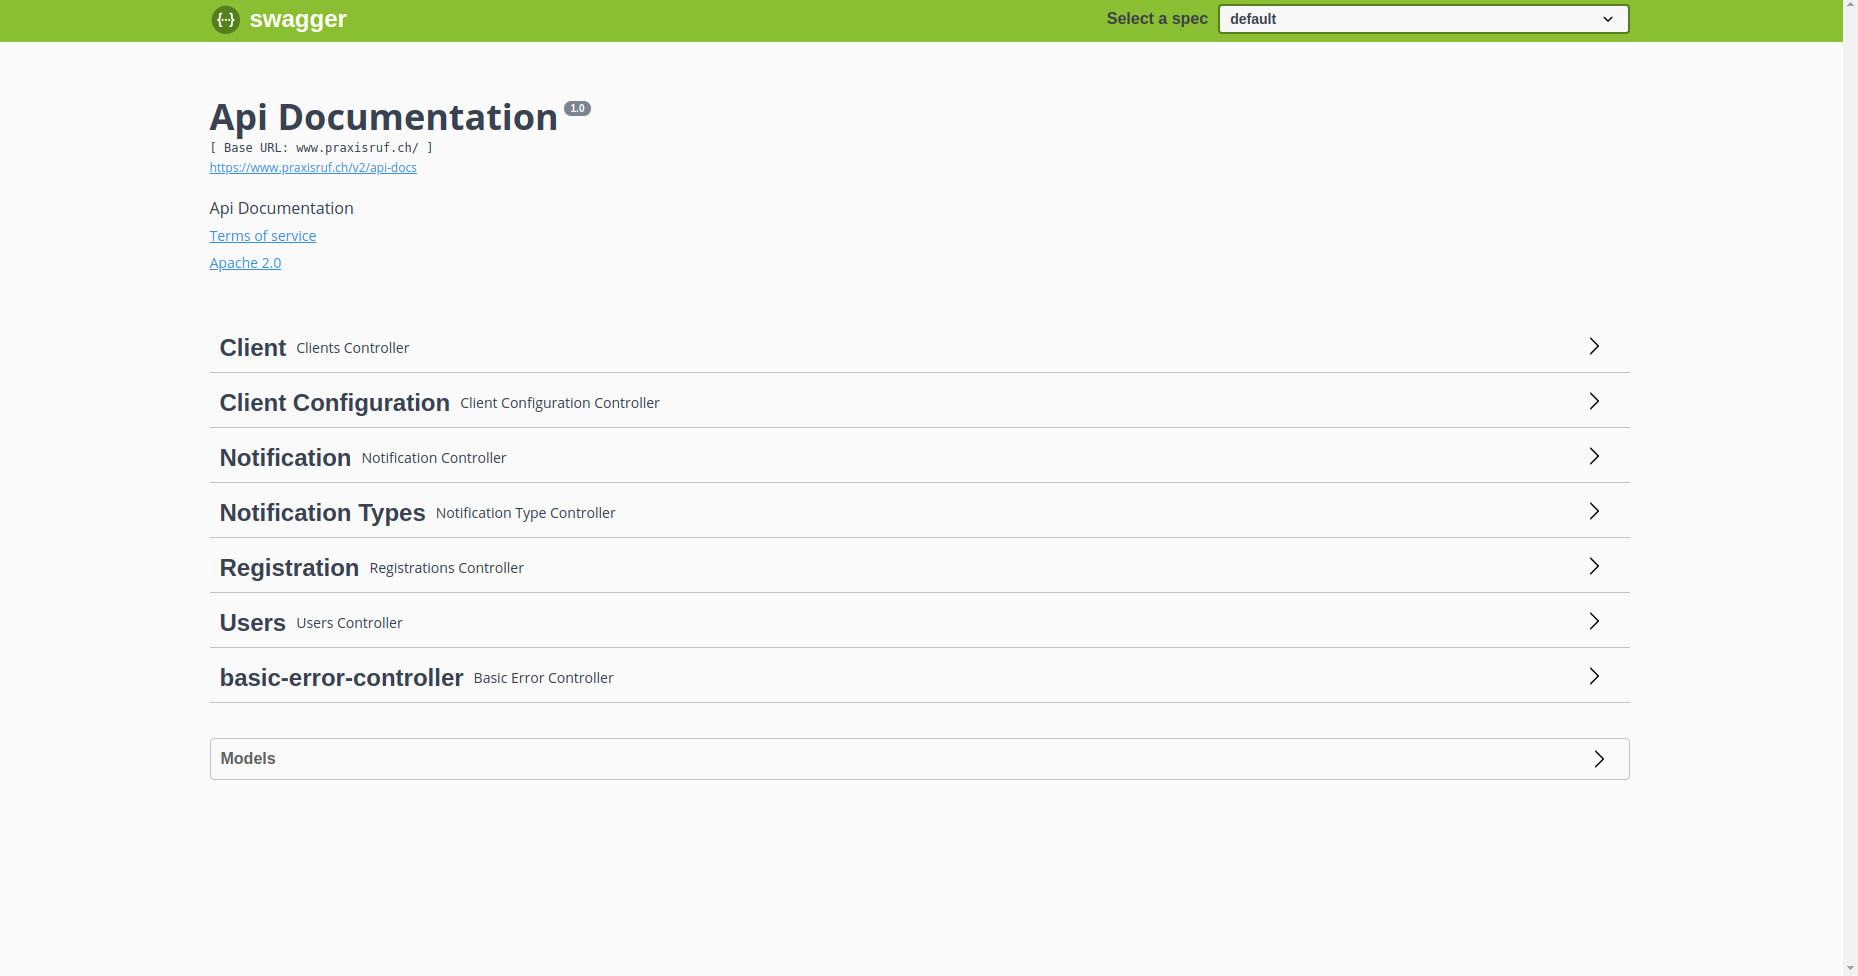
\includegraphics[width=\textwidth]{graphics/screenshots/cloud/swagger-home}
    \caption{Home}
\end{minipage}

Sorgt neben der API auch die Authentifikation die umgesetzt wurde.

\clearpage

\subsubsection{Admin UI}

\begin{figure}[h]
    \centering
    \begin{minipage}[b]{0.4\textwidth}
        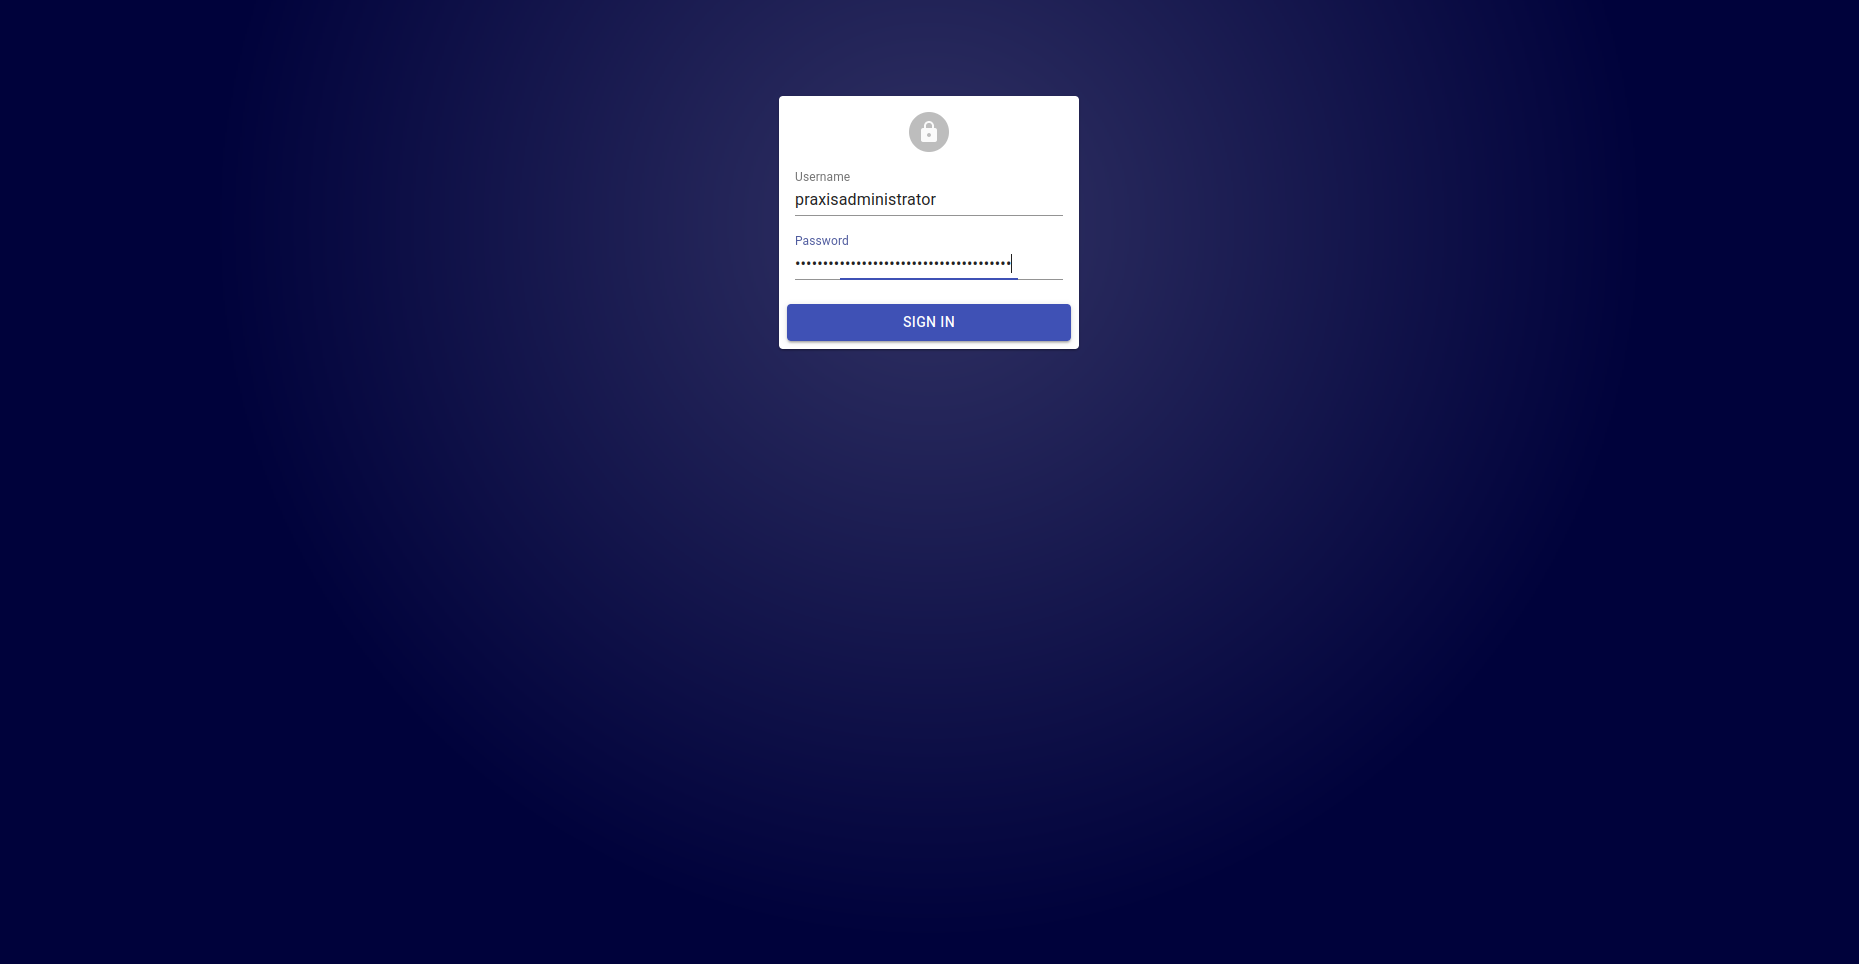
\includegraphics[width=\textwidth]{graphics/screenshots/adminui/login}
        \caption{Login}
    \end{minipage}
    \hfill
    \begin{minipage}[b]{0.4\textwidth}
        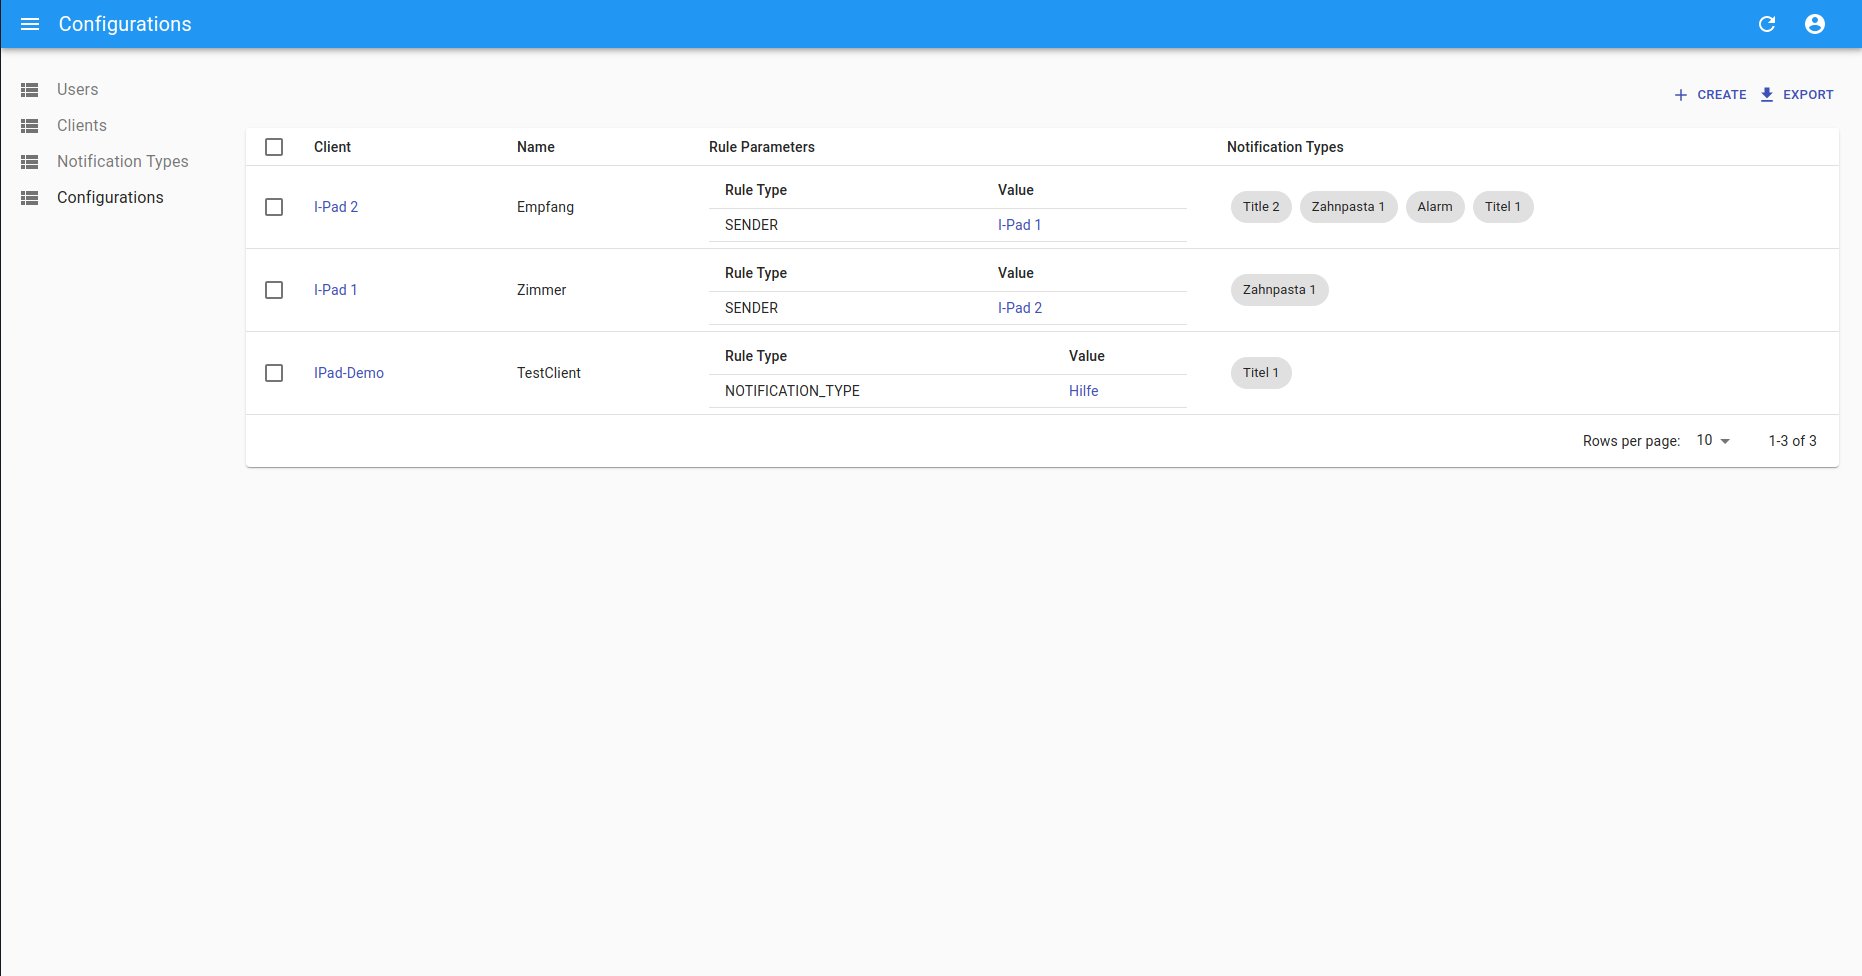
\includegraphics[width=\textwidth]{graphics/screenshots/adminui/configuration-all}
        \caption{Configuration Overview}
    \end{minipage}
    \label{fig:AdminUI-Screens1}
\end{figure}

\begin{figure}[h]
    \centering
    \begin{minipage}[b]{0.4\textwidth}
        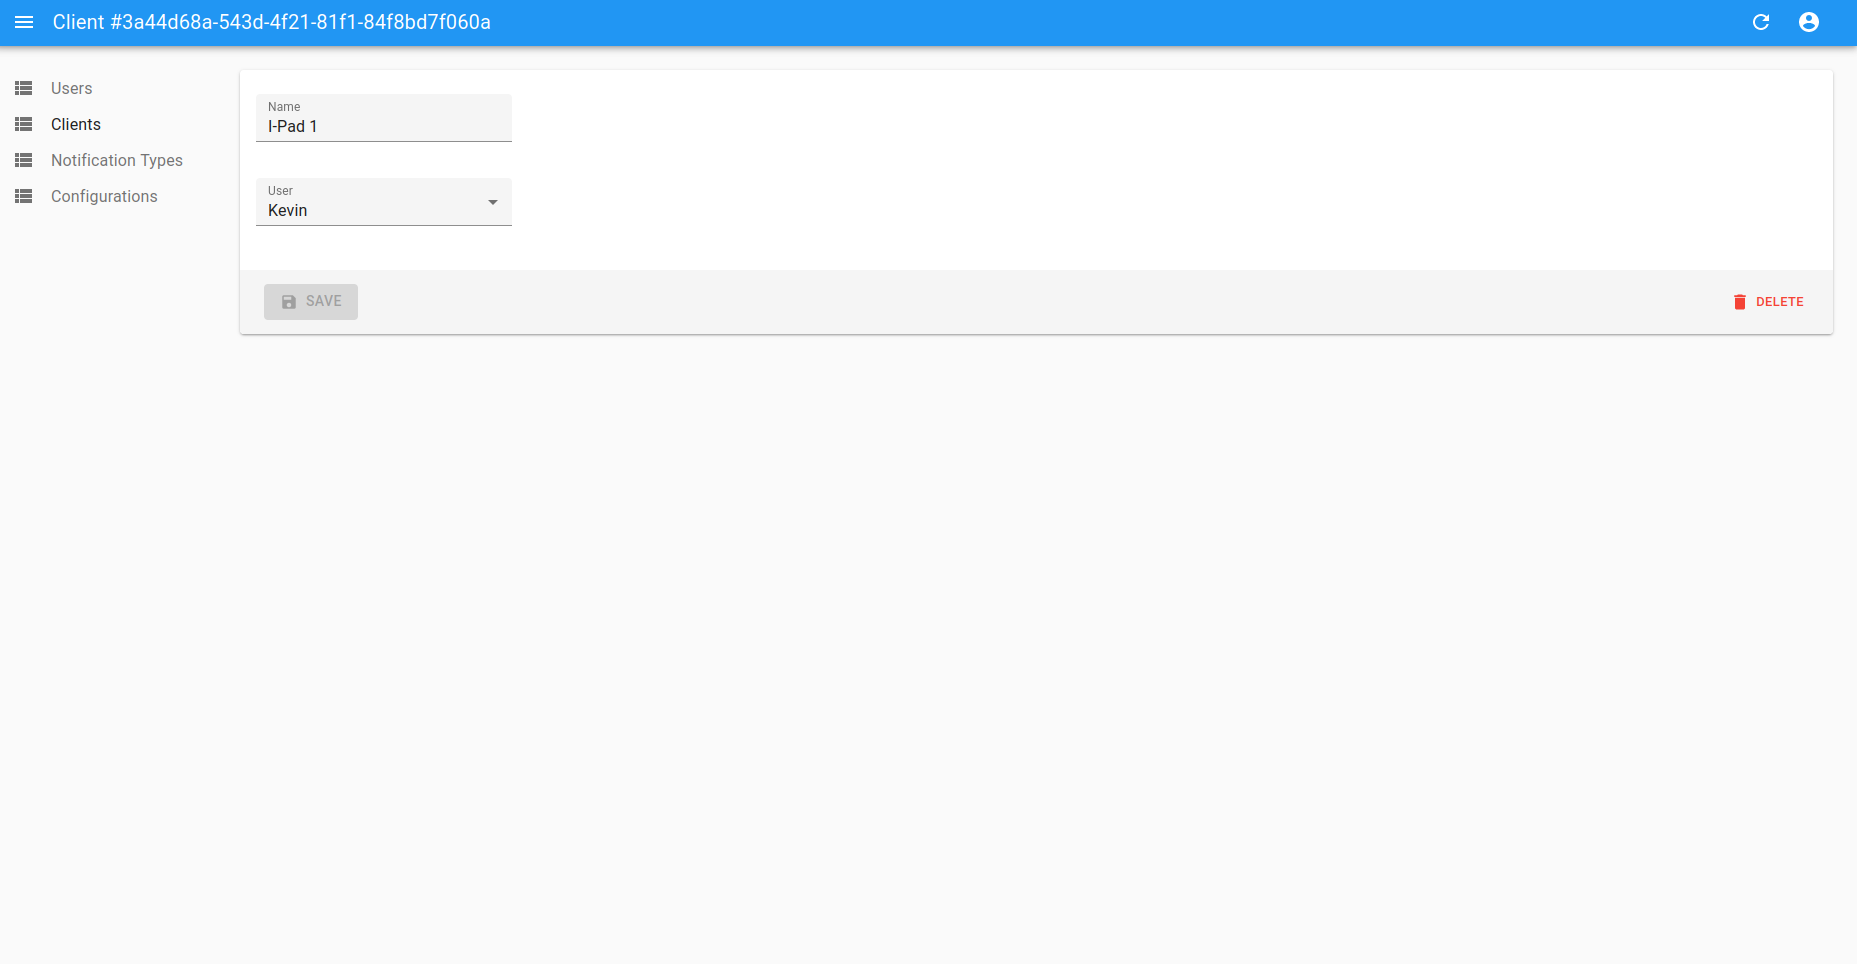
\includegraphics[width=\textwidth]{graphics/screenshots/adminui/configuration}
        \caption{Login}
    \end{minipage}
    \hfill
    \begin{minipage}[b]{0.4\textwidth}
        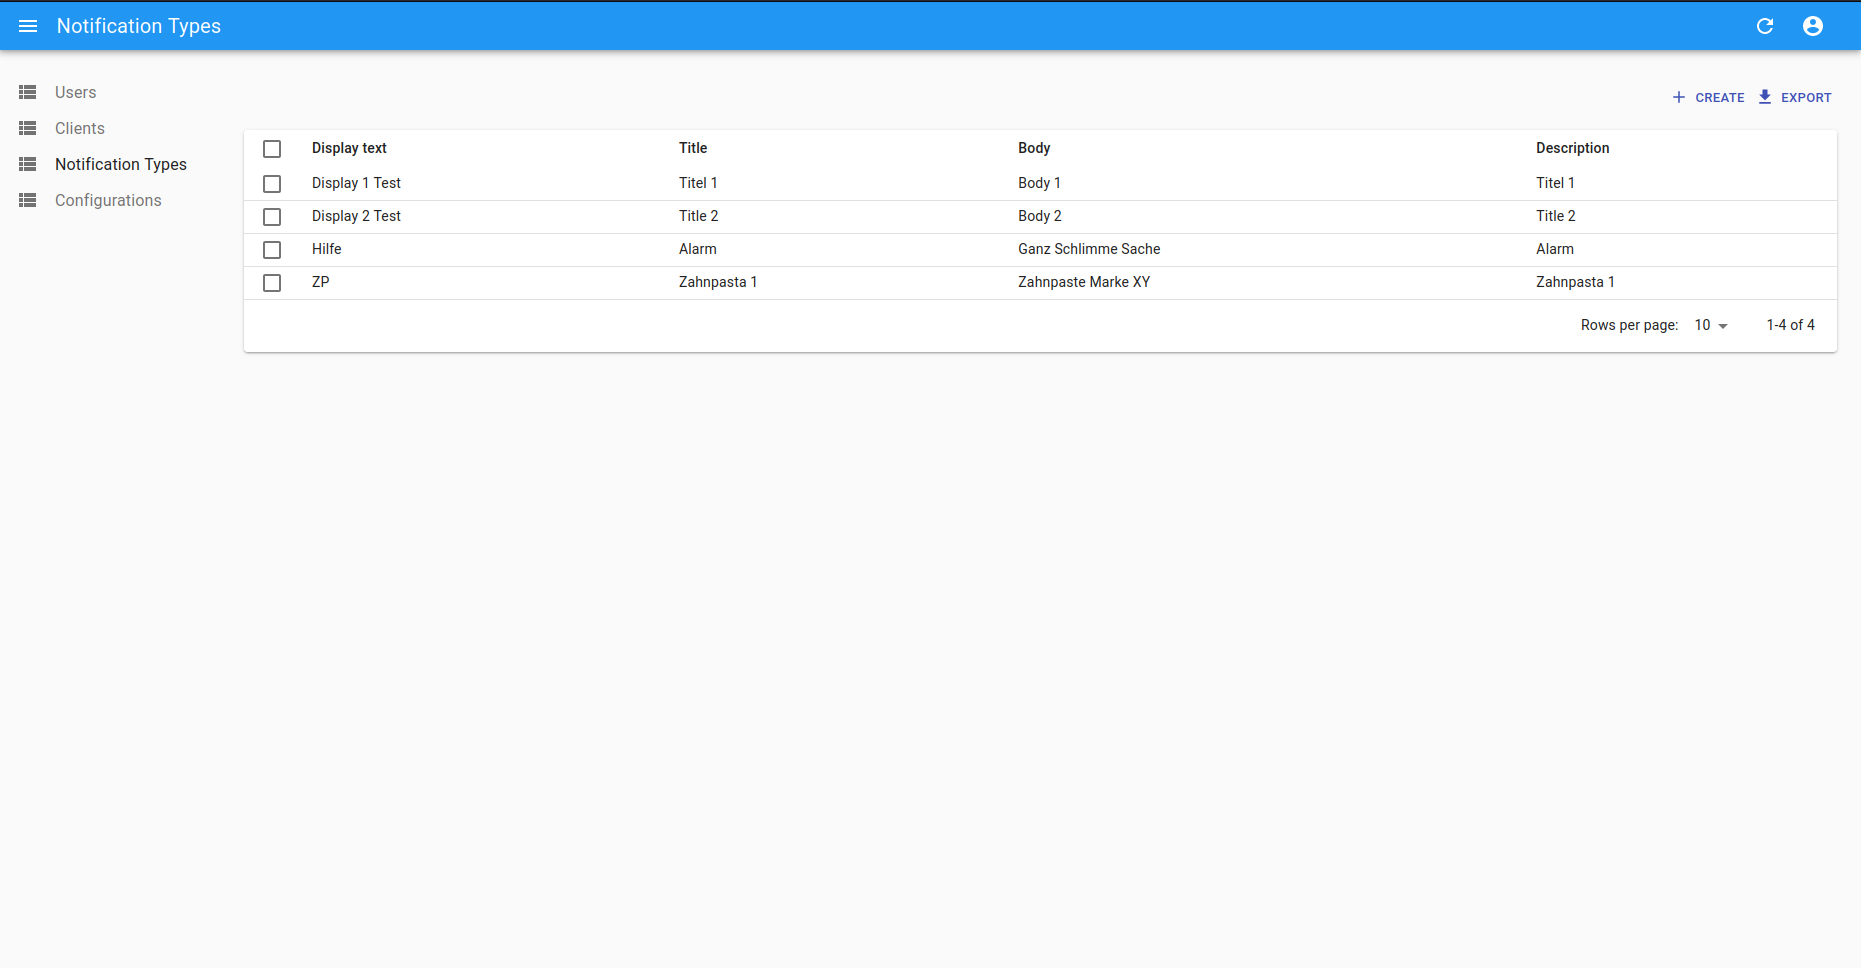
\includegraphics[width=\textwidth]{graphics/screenshots/adminui/notification-type}
        \caption{Configuration Overview}
    \end{minipage}
    \label{fig:AdminUI-Screens2}
\end{figure}




Add some screen shots

\subsection{Tests}

\subsubsection*{Benutzertests}
Wurden mit Daniel Jossen zusannem an der FH gemacht.
Mehr Tests waren wegen Ferienabwesenheiten auf Kundenseite nicht möglich.
Macht nicht so viel sinn mit nur einem Ipad.


\subsubsection*{Benutzertests}
Macht nicht so viel sinn mit nur einem Ipad.

\clearpage
\subsection{Lessons Learned}

\clearpage
\begin{itemize}
    \item Die Gegensprechanlage ist komplett Weggefallen.
    \subitem Grundsätzlich Stünde eine Lib. für IOS in NS zur Verfügung. Der Android Teil ist da noch "TODO"
    \item Die Rückfärbung der Buttons auf Grün ist weggefallen da der Handshake so nicht implmentiert wurde.
\end{itemize}


Hearusforderungen waren:
\begin{itemize}
    \item Dokumentation fehlt komplett in der Planung
    \item IOS Recherche viel aufwändiger als erwartet.
    \item Nativescript aufwändiger zu gebrauchen als erwartet.
    \item AWS aufsetzen ist alles andere als trivial
    \item Keine Erfahrung mit Mobile Development
    \item Stärkerer Roter Faden von Anfang an hätte geholfen
    \item Mehr testing, viel Mehr Testing.
    \item Refactoring kostet Zeit, kanns aber wert sein.
\end{itemize}

Darus mitgenommen haben wir:
\begin{itemize}
    \item Gute Planung macht sich bezahlt. (Roter Faden, Doku mit einplanen, Standortbestimmung)
    \item Gute Konzepte machen sich bezahlt.
    \item Best Practices gibt es aus einem Grund. (Nativ ist besser)
    \item DevOps ist schwer.
\end{itemize}





